%%
%% $Id$
%%
%% Copyright (c) 2007-2008 Christian Fehler
%% Copyright (c) 2007-2008 Benjamin Mies
%%


%### removes texlipse warnings


\chapter{Automaten}\label{Machines}

Im Mittelpunkt der Planung und der Umsetzung des \gtitools standen die Automaten.
Im Rahmen dieser Diplomarbeit wurden vier Automatentypen umgesetzt. Der
deterministische endliche Automat (DEA), der nichtdeterministische endliche
Automat (NDEA), der nichtdeterministische endliche Automat mit
$\epsilon$-Übergängen ($\epsilon$-NDEA) und schließlich der Kellerautomat. Die
verschiedenen Aspekte von Automaten werden in diesem Kapitel besprochen. Dazu
gehört die graphische Umsetzung, sowie die verschiedenen Möglichkeiten,
einen Automaten zu verwenden, nachdem er erstellt wurde.\vspace{10pt}


\section{Graphenansicht}\label{Graph}

In diesem Abschnitt wird die Graphendarstellung besprochen. Zu Beginn der
Diplomarbeit wurde diskutiert, welche Möglichkeiten zur Darstellung eines
Automaten zur Verfügung stehen. Im Raum standen das eigenständige
Implementieren der graphischen Komponenten, sowie die Verwendung einer
Bibliothek, die diese Funktionalität zur Verfügung stellt. Aufgrund des
vermutlich enormen Zeitaufwandes wurde entschieden, eine Bibliothek zu benutzen.
In Abschnit \ref{PerspectiveGraphics} wird darauf eingegangen, in wie weit eine
Änderung in Zukunft sinnvoll bzw. realisierbar wäre.\vspace{10pt} 

Da JGraph (siehe \cite{jgraph}) die benötigte Funktionalität zur Verfügung
stellt, um die Automaten darstellen zu können, wurde entschieden, diese
Bibliothek zu benutzen. Im Folgenden wird darauf eingegangen, wie Automaten mit
JGraph dargestellt werden und wie JGraph angepasst werden musste, um den
speziellen Ansprüchen unserer Umsetzung zu genügen.\vspace{10pt}


\subsection{Automatendarstellung mit JGraph}\label{GraphJGraph}

Bei der Darstellung der Automaten haben wir uns am Verlesungsskript \cite{Sieber}
orientiert. Wir wollten eine möglichst hohe Überdeckung erreichen, um
sicherzustellen, dass ein Benutzer einen existierenden Automaten verstehen kann,
ohne sich noch viel einlesen zu müssen. In den Vorlesungsunterlagen wird ein
Zustand als Kreis dargestellt. Ein akzeptierender Zustand wird über einen
doppelten Rahmen gekennzeichnet. Einen Startzustand erkennt man an einem Pfeil,
welcher mit Start beschriftet ist. In Abbildung \ref{FigureMachine} sieht man
wie ein Automat im GTI Tool dargestellt wird.\vspace{10pt}

\begin{figure}[h!]
\begin{center}
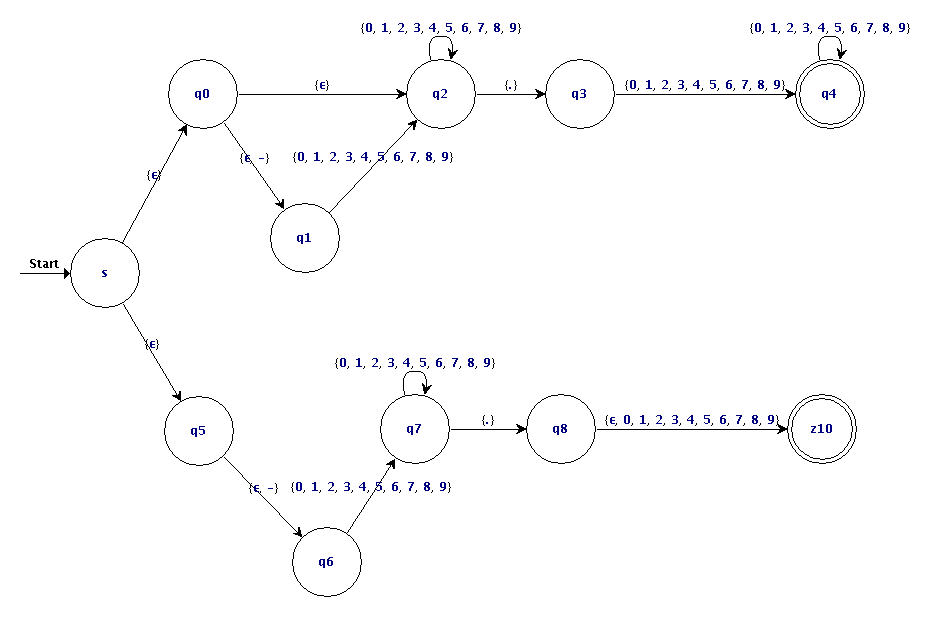
\includegraphics[width=12cm]{../images/enfa_example.png}
\caption{Beispiel für eine Automatendarstellung mit JGraph}
\label{FigureMachine}
\end{center}
\end{figure}
\vspace{10pt}

Als erstes mussten wir mit Hilfe von JGraph-Komponenten eine geeignete
Darstellung von Zuständen und Übergängen erreichen. Diese Komponenten müssen
dynamisch angelegt, gelöscht und bearbeitet werden können. Nachdem wir also eine
passende Darstellung für unsere Automaten gefunden hatten, mussten wir noch die
Verknüpfung von den graphischen Elementen und den eigentlichen Zustands- und
Übergangsobjekten herstellen. Um eine eindeutige Zuweisung von diesen Elementen
zu erreichen, haben wir uns dazu entschieden, die Kernelemente als Attribut in
den graphischen Komponenten zu speichern.\vspace{10pt}

Nachdem die Verknüpfung der Komponenten erledigt war, konnte man die Darstellung
der Zustände und Übergänge anhand der entsprechenden Daten anpassen. Für Zustände bedeutet
das, dass man den Namen des Zustandsobjekts anzeigt, und auswertet,
ob es sich um einen Startzustand oder um einen Endzustand handelt. Bei den
Übergängen konnte die Übergangsmenge als Beschriftung benutzt werden, wie es bei
der Vorlage im Skript der Fall ist.\vspace{10pt}


\subsection{Anpassung von JGraph}\label{GraphJGraphAdaptation}

Die Bibliothek JGraph bietet eine sehr weitreichende Unterstützung von
graphischen Komponenten. An einigen Stellen mussten allerdings Anpassungen
vorgenommen werden, um den von uns vorgegebenen Funktionumfang erreichen zu
können. Diese Anpassungen werden in diesem Abschnitt geschildert.\vspace{10pt}

Wir wollten in der Lage sein, die Farbe der Zustände je nach Situation
anzupassen, um zum Beispiel einen aktiven oder einen fehlerhaften Zustand anders
darzustellen. Dies wird zwar von der Bibliothek unterstützt, allerdings wurde von
uns eine Verknüpfung mit den Kernelementen gewünscht. Auf diese Weise ist es nun
möglich, einem solchen Kernelement zu sagen, dass es aktiv oder fehlerhaft ist.
Die graphische Komponente aktualisiert sich dann beim nächsten Zeichnen
automatisch. Durch diese Art der Implementierung ist es jetzt sehr einfach, in
den verschiedenen Algorithmen die Darstellung der graphischen Komponenten zu
beeinflussen.\vspace{10pt}

Eine weitere Anpassung, die von uns implementiert wurde, ist die Verwendung von
Pretty-Strings, welche in Abschnitt \ref{GUIDesign} bereits angesprochen wurde.
Diese Pretty-Strings werden zum Anzeigen der Namen verwendet, was gerade bei
Potenzautomaten-Zuständen einen Vorteil mit sich bringt, da die Namen der Zustände
aus denen der Potenzmengen-Zustand entstanden ist, besser hervorgehoben
werden.\vspace{10pt}

In Abschnitt \ref{ConverToMachine} wird die Umwandlung von Automaten in andere
Automaten- Formen, z.B. die Umwandlung von einem $\epsilon$-NDEA in einen DEA
besprochen. Bei der Implementierung dieser Umwandlung wurden wir vor das Problem
gestellt, dass in der Literatur Potenzautomaten-Zustände nicht rund dargestellt
werden, sondern als Rechteck mit abgerundeten Ecken. Dieses Problem wurde durch
die Anpassung der graphischen Zustände, sowie durch die Berechnung der Endpunkte
der Übergänge gelöst.\vspace{10pt}


\section{Tabellen}\label{Tables}

In diesem Abschnitt werden die zwei Tabellen beschrieben, die bei den Automaten
verwendet werden, um dem Benutzer zusätzliche Informationen zur Verfügung zu
stellen. Die Übergangstabelle bietet zusätzlich noch die Möglichkeit, den
Automaten zu verändern. Es können Übergänge angelegt, modifiziert oder gelöscht
werden.\vspace{10pt}


\subsection{Übergangstabelle}\label{TablesTransition}

Unter der {\em Übergangstabelle} versteht man eine Tabelle in der alle
Übergänge eingetragen sind. Abbildung \ref{FigureMachineTable} zeigt ein
Beispiel für eine solche Tabelle. In der ersten Spalte sind alle Zustände
aufgelistet. Die anderen Spalten beziehen sich jeweils auf das in der Kopfzeile
der Tabelle angegebene Symbol. In dem dargestellten Beispiel bedeutet der
Eintrag in der ersten Zeile, zweite Spalte, dass ein $\epsilon$-Übergang von
\State{z0} nach \State{z1} existiert.\vspace{10pt}

Während der Entwicklung und ersten Tests des \gtitools kam der Wunsch auf, einen
Automaten nicht nur graphisch zu bearbeiten, sondern auch in der
Übergangstabelle. Dadurch soll es dem Benutzer ermöglicht werden, Übergänge
schneller anzulegen, als es bei der normaler Methode in der Graphenansicht der
Fall wäre. Um diese neue Methode zu implementieren, wurden verschiedene
Umsetzungen diskutiert. Zur Diskussion standen unter anderem, dass in jeder Zelle
der Tabelle ausgewählt werden kann, zu welchen Zuständen ein Übergang existiert.
Diese Auswahl hätte allerdings bei der graphischen Umsetzung Probleme bereitet,
zumindest bei hinreichend vielen Zuständen. Aus diesem Grund wurde dieser Ansatz
verworfen.\vspace{10pt}

\begin{figure}[h!]
\begin{center}
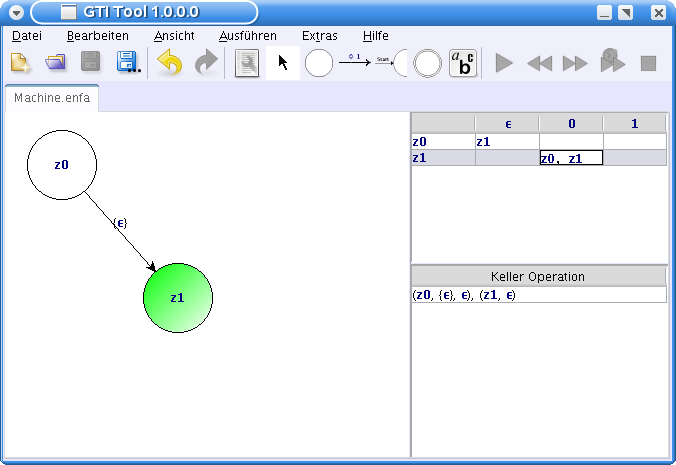
\includegraphics[width=12cm]{../images/machine_table.png}
\caption{Übergangstabelle}
\label{FigureMachineTable}
\end{center}
\end{figure}
\vspace{10pt}

Als nächste mögliche Umsetzung wurde diskutiert, ob es technisch möglich sei,
in jeder Zelle einen Parser zu verwenden. Dieser Parser müsste so implementiert
werden, dass er einen oder mehrere, durch Kommata getrennte Zustände als Eingabe
akzeptiert. Im Abschnitt \ref{Parser} wurden einige kontextsensitive Bedingungen
angesprochen, die auch bei dem hier vorliegenden Parser verwendet werden
mussten, da es dem Benutzer nicht möglich sein sollte, einen oder mehrere
Zustände anzugeben, die nicht im Graphen vorkommen. Abbildung
\ref{FigureMachineTable} zeigt das von uns umgesetzte Ergebnis.\vspace{10pt}


\subsection{Tabelle für Keller-Operationen}\label{TablesPDA}

Anhand der Tabelle für Kelleroperationen kann der Benutzer genau
nachvollziehen, was genau mit dem Keller des Automaten passiert, wenn dieser
in einen anderen Zustand übergeht.\vspace{10pt}

\begin{figure}[h!]
\begin{center}
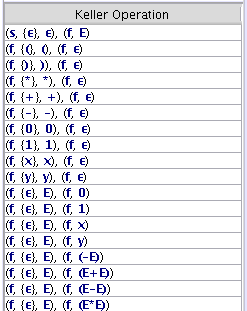
\includegraphics[width=12cm]{../images/stack_operation_table.png}
\caption{Tabelle für Keller-Operationen}
\label{FigureStackOperationTable}
\end{center}
\end{figure}
\vspace{10pt}

Die Tabelle enthält einen Eintrag pro Übergang in unserem Automaten. Jeder
Eintrag enthält den Ausgangszustand, den Folgezustand
und die entsprechende Übergangsmenge. Zusätzlich wird noch das Wort
angegeben, welches bei diesem Übergang vom Keller gelesen wird, und das Wort,
welches auf den Keller geschrieben wird. Wenn wir nichts vom Keller lesen, oder
auf den Keller schreiben, wird als Wort "`$\epsilon$"' verwendet. In Abbildung
\ref{FigureStackOperationTable} sieht man, wie eine solche Tabelle aussehen
kann.\vspace{10pt}


\section{Wort-Navigation}\label{WordNavigation}

In diesem Abschnitt wird die Wort-Navigation beschrieben. Neben der
deterministischen Navigation wird das Anzeigen des Pfades zu den aktuell
aktiven Zuständen angesprochen, das dem Benutzer erleichtern soll, zu
verstehen, warum ein eingegebenes Wort erkannt wird. Schließlich wird auf die
Operationen mit dem Automaten Keller eingegangen.


\subsection{Deterministische Navigation}\label{WordNavigationDeterministic}

Wir wollten dem Nutzer auch die Möglichkeit geben, sich anzusehen, wie der
konstruierte Automat ein beliebiges Eingabewort abarbeitet. Dabei muss es sich
um ein gültiges Wort über dem Alphabet handeln. Für diesen Zweck wurde die
Wort-Navigation entwickelt. In Abbildung \ref{FigureWordNavigation}
sieht man den Dialog zur WortNavigation im GTI Tool.\vspace{10pt}

Wenn der Nutzer den Wort-Navigationsmodus startet, findet er am unteren
Bildschirmrand zwei Textfelder. Hierbei handelt es sich um ein Eingabefeld für
das Eingabewort, und um eine Anzeige des aktuellen Kellers. In der
deterministischen Wort-Navigation spielt die Kelleranzeige keine Rolle. Diese
wird allerdings bei der Verwendung von einem Kellerautomaten benötigt und wird
in Abschnitt \ref{InteractionPDA} besprochen.\vspace{10pt}

Um dem Benutzer eine Hilfestellung bei der Eingabe eines Wortes zu geben, wird
rechts neben dem Eingabefeld das aktuelle Alphabet angezeigt. Man kann nur
Symbole verwenden, welche auch im Eingabealphabet enthalten
sind.\vspace{10pt}

\begin{figure}[h]
\begin{center}
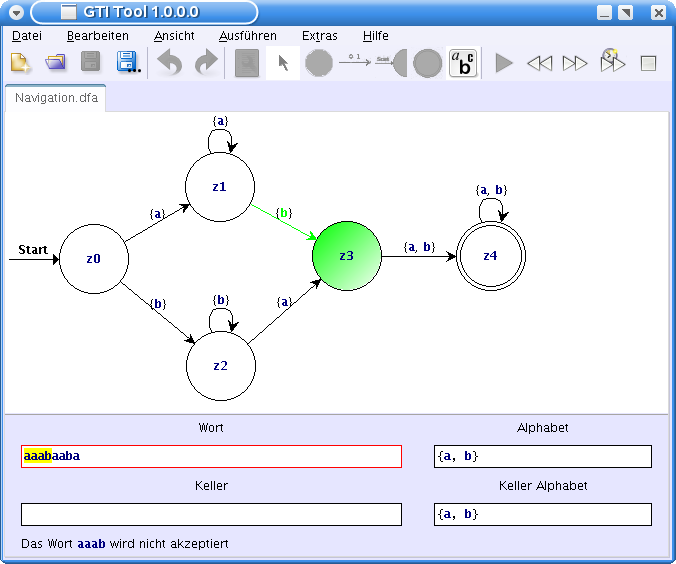
\includegraphics[width=12cm]{../images/dfa_navigation.png}
\caption{Automat - Wort-Navigation}
\label{FigureWordNavigation}
\end{center}
\end{figure}
\vspace{10pt}

Nachdem ein Wort eingegeben wurde, kann der Nutzer dann die Verarbeitung des
Worts starten. Es besteht die Möglichkeit, sich Zeichen für Zeichen weiter durch
das Wort zu arbeiten, und den genauen Weg im Automaten nachzuvollziehen.\vspace{10pt}

In jedem Schritt werden die Zustände farblich hervorgehoben, in denen sich der
Automat aktuell befindet. Zusätzlich wird auch der Übergang und das
entsprechende Symbol des Übergangs hervorgehoben, über welchen man in diesen
Zustand gekommen ist. In dem Feld, in welchem man das Wort eingegeben hat, wird
jetzt angezeigt, bis zu welcher Stelle der Automat das Wort schon gelesen
hat.\vspace{10pt}

Wenn der Automat das ganze Wort gelesen hat, bekommt der Benutzer eine Information,
ob der Automat das Wort akzeptiert hat, oder, ob das Wort nicht in der Sprache
des Automaten liegt.\vspace{10pt}


\subsection{Zustands Pfad}\label{HistoryPath}

Bei Verwendung eines nichtdeterministischen Automaten stellte sich bei der
Wort-Navigation die Frage, auf welchem Pfad die aktuell aktiven Zustände erreicht
wurden. Verschiedene Umsetzungen wurden von uns in Betracht gezogen, um dem
Benutzer die Ausgabe darzustellen. Es wurde schließlich entschieden, die Zustände
auf dem Pfad zu den aktuell aktiven Zuständen darzustellen. Auf diesem Pfad
werden die verwendeten Übergänge, sowie die verwendeten Symbole an den Übergängen
hervorgehoben. Da unter Umständen mehrere Pfade vorhanden sein können, werden
diese anhand der Anzahl der verwendeten Zustände sortiert, dabei werden die
kürzesten Pfade zuerst angezeigt.\vspace{10pt}

\begin{figure}[h!]
\begin{center}
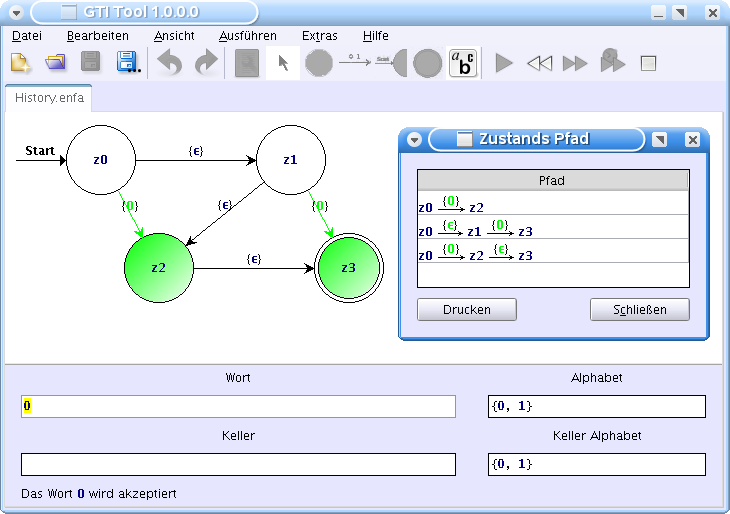
\includegraphics[width=12cm]{../images/history_path.png}
\caption{Zustands Pfad}
\label{FigureHistoryPath}
\end{center}
\end{figure}
\vspace{10pt}

Der implementierte Algorithmus geht rückwärts vor, startet also bei den aktuell
aktiven Zuständen und geht alle Pfade zurück, bis alle, beim Starten der Ansicht
vom Eingabewort gelesenen Symbole abgearbeitet sind. Startet der berechnete Pfad
dann in dem Startzustand, wurde ein gültiger Pfad erkannt. Bei der
Implementierung des Algorithmus musste eine Zykluserkennung umgesetzt werden, da
es sonst möglich wäre, in eine Endlosschleife zu geraten, welche durch
$\epsilon$-Übergänge verursacht wurde. Abbildung \ref{FigureHistoryPath} zeigt
ein einfaches Beispiel eines solchen Pfads.\vspace{10pt}


\subsection{Nichtdeterministische Kellerautomat-Navigation}\label{InteractionPDA}

Ein wichtiger Punkt ist, dass der Benutzer nach einer Umwandlung einer
kontextfreien Grammatik in einen Kellerautomaten einen Übergang auswählen muss,
wenn der entstehende Automat nicht deterministisch ist. Die eigentliche
Umwandlung ist in Abschnitt \ref{ConverToGrammarContextFree} zu
finden.\vspace{10pt}

\begin{figure}[h!]
\begin{center}
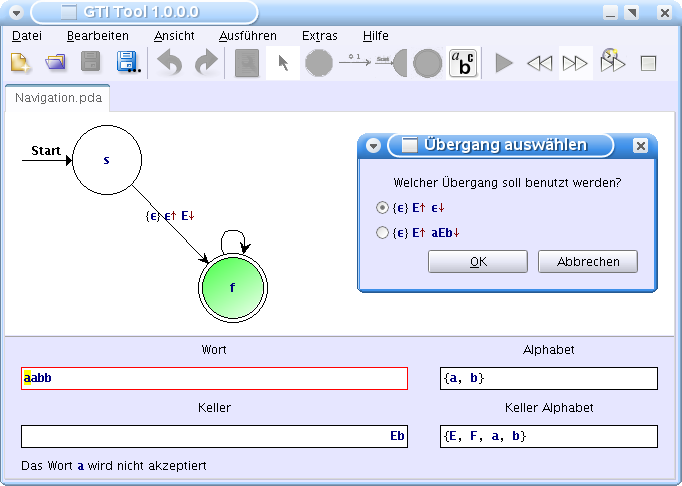
\includegraphics[width=12cm]{../images/grammar_pda.png}
\caption{Operationen mit dem Automaten Keller}
\label{FigureGrammarPDA}
\end{center}
\end{figure}
\vspace{10pt}

Bei dem in Abbildung \ref{FigureGrammarPDA} verwendeten Beispiel kommen zwei
Übergänge in Frage: Es könnte der Übergang gewählt werden, der \Symbol{E} vom
Keller liest und nichts auf diesen schreibt, oder aber der Übergang, der
\Symbol{E} vom Keller liest und \Symbol{a}\Symbol{E}\Symbol{b} auf ihn schreibt.
Da \Symbol{a} als nächstes auf dem Eingabeband steht, sollte der zweite Übergang
ausgewählt werden, da bei der Verwendung des ersten Übergangs das \Symbol{a}
nicht mehr herleitbar ist. Dem Benutzer steht es allerdings frei, auch den
anderen Übergang auszuwählen. In diesem Fall würde das Wort
\Symbol{a}\Symbol{a}\Symbol{b}\Symbol{b} aber nicht akzeptiert werden. Der
Benutzer hat bei einer Wahl, die sich im Nachhinein als falsch herausstellt,
allerdings die Möglichkeit, einen oder mehrere Schritte zurückzugehen, um dann
die hoffentlich richtige Wahl zu treffen.\vspace{10pt}


\section{Erreichbare Zustände}\label{ReachableStates}

Nach dem in \ref{ConverToMachine} angesprochenen Umwandeln eines
nichtdeterministischen in einen deterministischen Automaten unter Verwendung der
Potenzautomatenkonstruktion stellte sich die Frage, wie die unerreichbaren
Zustände erkannt und entfernt werden können. Dieses Problem betrifft aber nicht
nur umgewandelte Automaten, sondern ganz allgemein, jeden erstellten
Automaten.\vspace{10pt}

Bei der Umsetzung sollte im Vordergrund stehen, dass dem Benutzer mit sehr
kleinen Schritten verdeutlicht wird, wie der zugrundeliegende Algorithmus
arbeitet, so dass diese Arbeitsweise sehr einfach nachzuvollziehen
ist.\vspace{10pt}

Zur Umsetzung wurde der in \cite[S. 536]{Algorithmen} angegebene Algorithmus
als Vorlage benutzt. Dieser Algorithmus implementiert die Breitensuche auf
einem Graphen G mit Startknoten s. Zur Interpretation des Algorithmus ist noch
zu sagen, dass das Attribut Farbe eines Knoten dazu verwendet wird, zu
speichern, in welcher Phase des Algorithmus er sich befindet. Ist ein Knoten
weiß, bedeutet das, dass er noch nicht erkannt wurde. Am Anfang sind alle
Knoten, außer dem Startknoten, weiß. Grau bedeutet, dass der Knoten erkannt
wurde, aber noch nicht vollständig abgearbeitet wurde. Wurde ein Knoten
abgearbeitet, ändert sich seine Farbe in schwarz. Bei der Umsetzung im \gtitool
wurde eine ähnliche Umsetzung gewählt, die nun dargestellt wird.\vspace{10pt}

\noindent
\verb| 1 BFS(G,s)|\\
\verb| 2 for alle Knoten u |$\in$\verb| V[G] - {s}|\\
\verb| 3     do farbe[u] |$\gets$\verb| WEISS|\\
\verb| 4        d[u] |$\gets \infty$\\
\verb| 5        |$\pi$\verb|[u] |$\gets$\verb| NIL|\\
\verb| 6 farbe[s] |$\gets$\verb| GRAU|\\
\verb| 7 d[s] |$\gets$\verb| 0|\\
\verb| 8 |$\pi$\verb|[s] |$\gets$\verb| NIL|\\
\verb| 9 Q |$\gets \emptyset$\\
\verb|10 ENQUEUE(Q,s)|\\
\verb|11 while Q |$\neq \emptyset$\\
\verb|12       do u |$\gets$\verb| DEQUEUE(Q)|\\
\verb|13          for alle v |$\in$\verb| Adj[u]|\\
\verb|14              do if farbe[v] = WEISS|\\
\verb|15                    then farbe[v] |$\gets$\verb| GRAU|\\
\verb|16                         d[v] |$\gets$\verb| d[u] + 1|\\
\verb|17                         |$\pi$\verb|[v] |$\gets$\verb| u|\\
\verb|18                         ENQUEUE(Q,v)|\\
\verb|19          farbe[u] |$\gets$\verb| SCHWARZ|\\
\vspace{10pt}

Der dann im Programm umgesetzte Algorithmus besteht aus drei Phasen. Abbildung
\ref{FigureReachableStates} zeigt ein einfaches Beispiel der erreichbaren
Zustände.\vspace{10pt}

In der ersten Phase wird ein noch nicht abgearbeiteter Zustand ausgewählt, also
ein Zustand, der von einem anderen Zustand aus erreichbar ist, aber für den noch
nicht berechnet wurde, welche Zustände von ihm aus erreichbar sind. Zu Beginn des
Algorithmus wird mit dem Startzustand angefangen. In der zweiten Phase werden die
von diesem Zustand aus direkt erreichbaren Zustände berechnet und dem Benutzer
hervorgehoben dargestellt. In der dritten Phase werden alle bis jetzt
erreichbaren Zustände hervorgehoben. Gleichzeitig wird rechts in der Outline
angezeigt, welcher Zustand jetzt fertiggestellt ist und welche noch berechnet
werden müssen. Durch diese sehr feine Unterteilung soll ein besseres Verständnis
des Algorithmus erreicht werden.\vspace{10pt}

\begin{figure}[h!]
\begin{center}
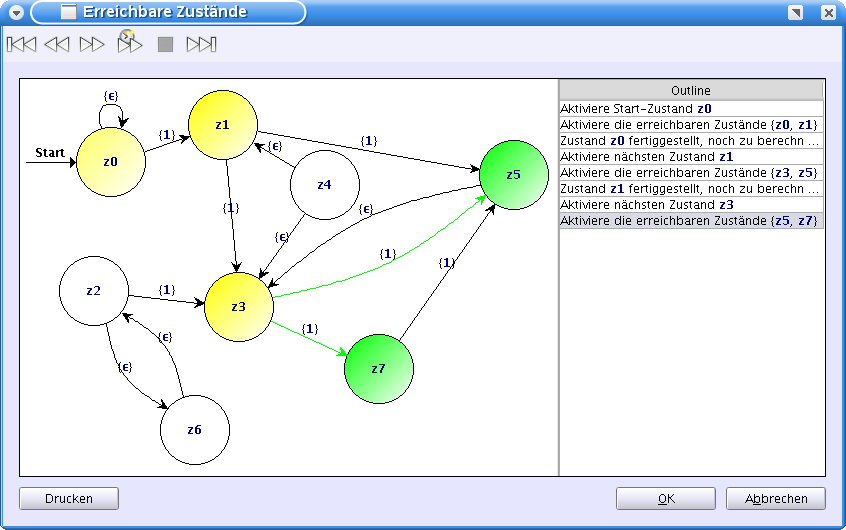
\includegraphics[width=12cm]{../images/reachable_states.png}
\caption{Erreichbare Zustände}
\label{FigureReachableStates}
\end{center}
\end{figure}
\vspace{10pt}


\section{Konvertierung}\label{ConverToMachine}

Bei der Planung der Umwandlung zwischen den verschiedenen Automatentypen stellte
sich die Frage, wie dem Benutzer der Umwandlungsalgorithmus möglichst
verständlich dargestellt wird. Aus diesem Grund wurde die in Abschnitt
\ref{GUIDesign} angesprochene Navigationsleiste verwendet.\vspace{10pt}

Um dem Benutzer den durchgeführten Algorithmus zu verdeutlichen, wurde die
Ansicht in drei Bereiche eingeteilt. In dem oberen linken Bereich wird der
Ausgangsautomat dargestellt, im unteren linken Bereich der nach und nach
entstehende konvertierte Automat und schließlich im rechten Bereich eine Outline,
die pro Ausführungsphase, jeweils mit einem Kommentar, angibt, welchen Schritt
der Algorithmus im Moment durchführt.\vspace{10pt}

\begin{figure}[h!]
\begin{center}
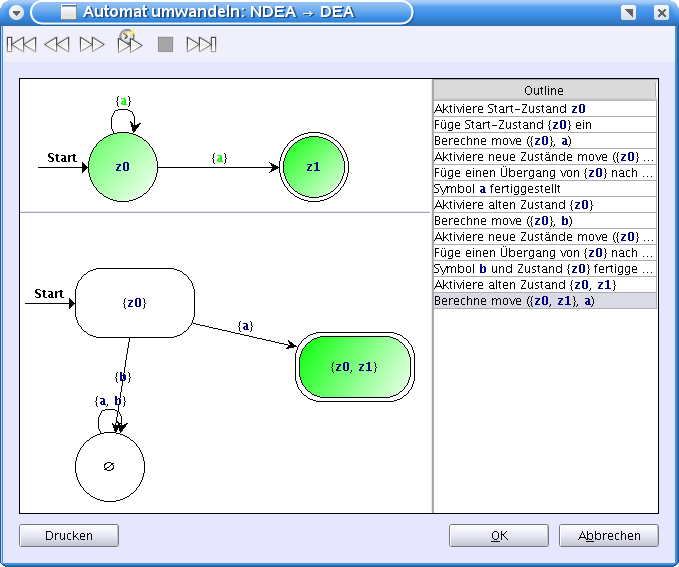
\includegraphics[width=12cm]{../images/convert_to.png}
\caption{Automat umwandeln}
\label{FigureConvertTo}
\end{center}
\end{figure}
\vspace{10pt}

Es existieren zwei verschiedene Verfahren zur Umwandlung eines
nichtdeterministischen endlichen Automaten in einen deterministischen endlichen
Automaten (DEA). Zum einen kann der komplette Potenzautomat verwendet werden, um
den DEA zu erzeugen. Der entstehende Automat enthält allerdings unter Umständen
sehr viele nicht erreichbare Zustände, deren Berechnung einige zusätzliche
Schritte zur Folge haben kann. Wenn der Benutzer diese Art der Umwandlung
auswählt, kann er nach dem Umwandeln die nicht erreichbaren Zustände wieder
entfernen. Wie dies funktioniert, kann in \ref{ReachableStates} nachgelesen
werden. Die zweite Methode ist, dass nur die erreichbaren Zustände in der unteren
Ansicht angelegt werden. Diese Methode ist übersichtlicher für den Benutzer, wenn
auch nicht alle im Potenzautomaten vorhandenen Zustände betrachtet
werden.\vspace{10pt}

\newpage
Zur Umsetzung wurde der in \cite[S. 153ff]{Compilers} angegebene Algorithmus als
Vorlage benutzt. Um den Algorithmus verstehen zu können, müssen zuerst einige
Terme definiert werden.\vspace{10pt}

\noindent
\begin{tabular}{|p{2.2cm}|p{9.0cm}|}
  \hline
  NFA A                 & Input NFA \\
  \hline
  DFA D                 & Output DFA \\
  \hline
  Dstates               & States of output DFA D \\
  \hline
  Dtran                 & Transition function of DFA D \\
  \hline
  $\epsilon$-closure(s) & Set of NFA states reachable from NFA state s
                          on $\epsilon$-transitions alone \\
  \hline
  $\epsilon$-closure(T) & Set of NFA states reachable from some NFA state s
                          in set T on $\epsilon$-transitions alone; =
                          $\cup_{s\ in\ T}\ \epsilon$-closure(s). \\
  \hline
  move(T,a)             & Set of NFA states to which there is a transition
                          on input symbol a from some state s in T \\
  \hline
\end{tabular}
\vspace{10pt}

Abbildung \ref{FigureConvertTo} zeigt die Umwandlung nach einigen Schritten. Die
eigentliche Umwandlung geschieht dann mit folgendem Algorithmus:\vspace{10pt}

\noindent
\verb| 1 initially, |$\epsilon$\verb|-closure(|$s_0$\verb|) is the only state in Dstates,|\\
\verb| 2 and it is unmarked;|\\
\verb| 3 while ( there is an unmarked state T in Dstates ) {|\\
\verb| 4       mark T;|\\
\verb| 5       for ( each input symbol a ) {|\\
\verb| 6           U = |$\epsilon$\verb|-closure(move(T,a));|\\
\verb| 7           if ( U is not in Dstates )|\\
\verb| 8              add U as an unmarked state to Dstates;|\\
\verb| 9           Dtran[T,a] = U;|\\
\verb|10       }|\\
\verb|11 }|
\vspace{10pt}

Dieser Algorithmus verwaltet eine Menge \textit{Dstates} von Zuständen des
umgewandelten Automaten. Neben dieser Menge wird für jeden Zustand gespeichert,
ob er schon verarbeitet wurde. Am Anfang wird der $\epsilon$-Abschluss des
Start-Zustandes \State{$s_0$} in die Menge \textit{Dstates} aufgenommen. In Zeile
vier wird der aktuelle Zustand markiert, jeder neue Zustand in \textit{Dstates}
wird somit abgearbeitet. In der Schleife in Zeile fünf wird über alle Symbole des
Alphabets iteriert. In Zeile sechs wird berechnet, welche Zustände von dem
aktuellen Symbol aus erreichbar sind, zusätzlich dazu wird von diesem Ergebnis
noch der $\epsilon$-Abschluss berechnet. Anschließend wird dieser neue Zustand zu
der Menge \textit{Dstates} hinzugefügt, falls er noch nicht enthalten ist.
Außerdem wird der Zustand in diesem Fall als nicht markiert gekennzeichnet.
Abschließend wird in Zeile neun die neue Übergangsfunktion
gespeichert.\vspace{10pt}


\section{Minimierung}\label{Minimize}

Sobald der Benutzer einen Automaten erstellt hat, kann er mit diesem schon alle
Funktionen, welche dieses Lernwerkzeug bietet, nutzen. Allerdings besteht die
Möglichkeit, dass ein Automat existiert, der die gleiche Sprache erkennt, die ein
erstellter Automat erkennt, jedoch mit weniger Zuständen auskommt. Bei
komplexeren Beispielen bemerkt man schnell, dass die Übersichtlichkeit mit
wachsender Anzahl der Zustände immer weiter abnimmt. Daher ist es wünschenswert,
immer mit dem minimalen Automaten für eine bestimmte Sprache zu arbeiten. Im
Folgenden wollen wir uns jetzt den Algorithmus ansehen, welcher verwendet wird,
um aus einem Automaten einen neuen Automaten mit einer minimalen Anzahl von
Zuständen zu erzeugen. Dieser Algorithmus ist aus \cite{Compilers}
entnommen. In Abbildung \ref{FigureMinimization} sieht man wie die
Minimierung im GTI Tool graphisch dargestellt wird.\vspace{10pt}

Wie bereits erwähnt, erwartet der Algorithmus als Eingabe einen Automaten, und
erzeugt als Ausgabe einen neuen Automaten welcher die gleiche Sprache
akzeptiert, jedoch mit einer minimalen Anzahl von Zuständen
auskommt.\vspace{10pt}

Der erster Minimierungsschritt besteht darin, die unerreichbaren Zustände zu
entfernen, da diese keine Auswirkung auf die erkannte Sprache haben können. Der
dazu verwendete Algorithmus zur Berechnung der erreichbaren Zustände kann im
Abschnitt \ref{ReachableStates} nachgeschlagen werden.\vspace{10pt}

Im Weiteren versuchen wir, äquivalente Zustände in Gruppen, auch
Äquivalenz\-klassen genannt, zusammenzufassen, um diese später zu einem Zustand
zu verschmelzen. Um herauszufinden, ob zwei Zustände in der gleichen
Äquivalenz\-klasse liegen, überprüft man für jedes Symbol des Alphabets
einzeln, ob alle Zustände der Gruppe mit diesem Symbol in Zustände der selben
Gruppe übergehen.\vspace{10pt}

Initial wird unsere Menge von Zuständen in zwei Gruppen unterteilt. Alle
akzeptierenden Zustände bilden die erste, alle nicht akzeptierenden Zustände die
zweite Gruppe.\vspace{10pt}

Der Algorithmus nimmt sich jetzt das Alphabet des Eingabeautomaten zur Hilfe, um
zu prüfen, ob alle Zustände einer Gruppe wirklich in einer Äquivalenzklasse
liegen, oder ob wir die Gruppe aufspalten müssen. Dazu sei gesagt, dass zwei
Zustände in der selben Äquivalenzklasse liegen, wenn sie mit jeweils allen
Symbolen des Eingabealphabets in einen Zustand der selben Gruppe
übergehen.\vspace{10pt}

\begin{figure}[h]
\begin{center}
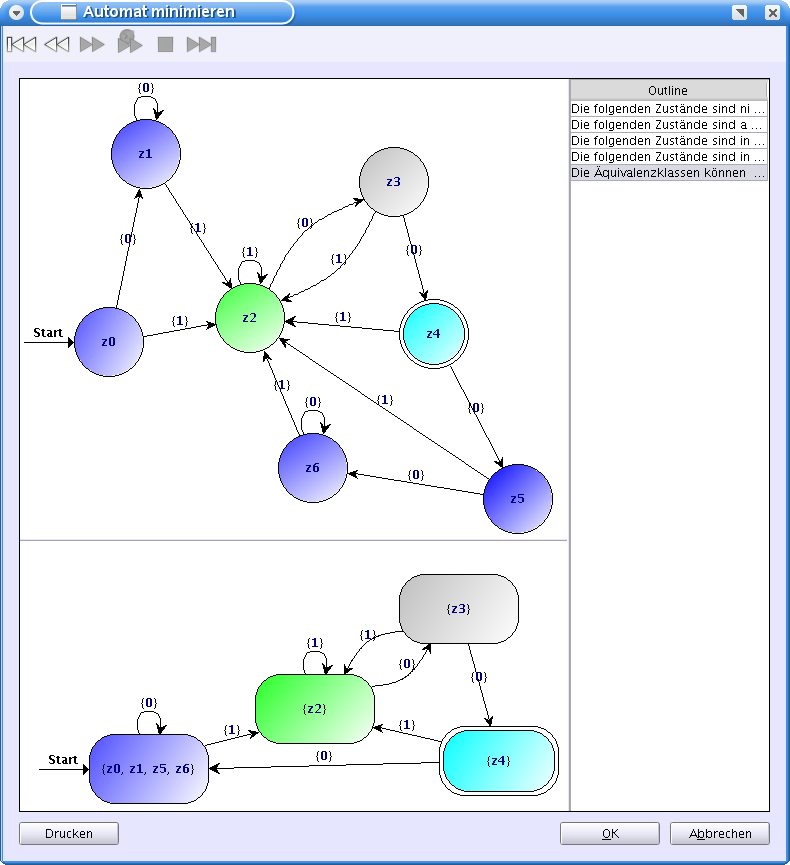
\includegraphics[width=12cm]{../images/minimize.png}
\caption{Automat - Minimierung}
\label{FigureMinimization}
\end{center}
\end{figure}
\vspace{10pt}

Schauen wir uns jetzt mal die Arbeitsweise des Algorithmus im Detail an. Als
erstes wird die aktuelle Gruppeneinteilung gespeichert, also wie viele
Gruppen existieren, und welcher Zustand in welcher Gruppe liegt. Dann wird
die erste Gruppen betrachtet. Wenn diese nur einen Zustand enthält, kann sie
nicht weiter verfeinert werden, und muss daher auch nicht mehr betrachtet werden.
\vspace{10pt}

Enthält die Gruppe mehr als einen Zustand, wird das aktuelle Alphabet des
Automaten betrachtet. Der Algorithmus überprüft jetzt, ob alle Zustände dieser
Gruppe in der gleichen Äquivalenzklasse liegen. Wenn das der Fall ist, kann auch
diese Gruppe nicht weiter unterteilt werden. Falls aber doch Zustände
existieren, welche in einer anderen Äquivalenz\-klasse liegen, werden diese
Zustände aus der aktuellen Gruppe entfernt und bilden eine neue Gruppe. \vspace{10pt}

Nachdem diese Prozedur für die aktuelle Gruppe abgeschlossen ist, wird sie für
alle Gruppen, die noch nicht betrachtet wurden, wiederholt. Nach Betrachtung aller
Gruppen wird die aktuelle Gruppeneinteilung mit der verglichen, die zu Beginn
gespeichert wurde. Wenn diese übereinstimmt, ist unser Algorithmus am Ende, und
die Gruppen können nicht weiter verfeinert werden. Stimmt die Gruppeneinteilung
nicht überein, muss jede Gruppe erneut einzeln betrachten, um zu versuchen,
diese in kleinere Gruppen zu zerlegen.\vspace{10pt}

Nach Beendigung des Algorithmus repräsentiert jede Gruppe einen Zustand
im minimalen Automaten. Jetzt muss noch pro Symbol des Alphabets der
Übergang in den entsprechenden neuen Zustand angelegt werden. Mit diesem
letzten Schritt ist die Konstruktion des minimalen Automaten
abgeschlossen.\vspace{10pt}

In unserem Lernwerkzeug wird dem Benutzer wie üblich in der Outline angezeigt,
was in den bisherigen Schritten des Algorithmus passiert ist.\vspace{10pt}


\section{Auto-Layout}\label{AutoLayout}

Beim Anlegen eines neuen Automaten, oder auch beim Modifizieren eines
bestehenden, kommt es vor, dass die Übersichtlichkeit verloren geht. Damit man
eine schnelle Möglichkeit hat, den Automaten wieder besser überblicken zu
können, wurde eine Auto-Layout Funktion implementiert.\vspace{10pt}

Diese Funktion basiert zur Zeit auf dem Erweiterten Partitionierungsalgorithmus
von Kerninghan und Lin. Er beruht auf der iterativen Verbesserung durch
paarweisen Austausch.\vspace{10pt}

Dieser Algorithmus wird eigentlich für die Partitionierung von Schaltungen auf
einem Verdrahtungsträger verwendet. Dabei soll es zu möglichst wenig
Überschneidungen der Leiterbahnen kommen, weil die Leiterbahnen dann auf mehrere
Ebenen verteilt werden müssen. Der Kerninhan-Lin Algorithmus kann aber problemlos
auf unsere Situation übertragen werden. Allerdings mussten bei der Übertragung
einige Modifikationen vorgenommen werden, auf welche wir später noch näher
eingehen werden.\vspace{10pt}


\subsection{Der Kerninghan-Lin-Algorithmus}\label{KerninghanLin}

Zu Beginn wird das Partitionierungsproblem in eine Graphendarstellung
transformiert. Danach wird die Knotenmenge V in zwei Gruppen, mit jeweils n
Elementen unterteilt. Anschließend werden für die aktuelle Einteilung die Kosten
berechnet. Als Kosten bezeichnen wir Schnitte mit einer imaginären Linie
zwischen zwei Gruppen.\vspace{10pt}

In jedem Durchlauf wird mehrfach ein Gewinnwert $\Delta g$ berechnet. Einen
Gewinnwert kann man erreichen, indem man zwei Knoten austauscht, und dadurch
die Anzahl der Schnitte verringert, wobei der Gewinnwert der Differenz
zwischen der neuen und alten Anzahl von Schnitten entspricht.

Der Kerninghan-Lin-Algorithmus lässt sich in die folgenden Schritte
unterteilen, welche dem Buch "`Layoutsynthese elektronischer
Schaltungen"' \cite{Layout} entnommen wurden:\vspace{10pt}

Schritt 1:
\begin{itemize}
  \item i=1
  \item Berechnung von D(v) für alle Knoten v $\in$ V
\end{itemize}

Schritt 2:
\begin{itemize}
  \item Auswahl von $a_i$ und $b_i$ mit maximalem Gewinnwert $\Delta g_i =
  D(a_i) + D(b_i) - 2 * c(a_i b_i)$
  \item Vertauschen und fixieren von $a_i$ und $b_i$
\end{itemize}


Schritt 3:
\begin{itemize}
  \item Wenn alle Knoten fixiert sind, weiter mit Schritt 4, andernfalls
  \item Neuberechnung der D-Werte für alle Knoten, welche nicht fixiert und
  mit $a_i$ und $b_i$ verunden sind
  \item i=i+1
  \item Weiter mit Schritt 2
\end{itemize}

Schritt 4:
\begin{itemize}
  \item Bestimmung der Vertauschungssequenz 1 bis m $(1 \leq m \leq i)$, so dass
  $G_m = \sum_{i=1}^{m}{\Delta g_i}$ maximiert wird
  \item Wenn $G_m > 0$, weiter mit Schritt 5, andernfalls ENDE
\end{itemize}

Schritt 5:
\begin{itemize}
  \item Durchführen aller m Vertauschungen, beseitigen aller Knotenfixierungen
  \item Weiter mit Schritt 1
\end{itemize}\vspace{10pt}

Betrachten wir zunächst, wie der Algorithmus vorgeht, indem wir
nachvollziehen, was in den einzelnen Schritten passiert.\vspace{10pt}

In \textit{Schritt 1} wird für alle Knoten berechnet, ob sie einen hohen oder
niedrigen Anteil der Schnittkosten verursachen. Die beiden Knoten, welche den
maximalen Gewinnwert bringen, werden getauscht und fixiert.\vspace{10pt}

In \textit{Schritt 3} überprüfen wir, ob alle Knoten bereits fixiert sind,
ansonsten werden die Kosten für jeden Knoten der noch nicht fixiert ist neu
berechnet und erneut
\textit{Schritt 2} ausgeführt.\vspace{10pt}

In \textit{Schritt 4} wird überprüft, ob der Algorithmus bereits sein Ende
erreicht hat. Wenn nicht, werden in \textit{Schritt 5} die Vertauschungen des
aktuellen Durchgangs durchgeführt, und es wird ein neuer Durchgang gestartet.\vspace{10pt}

Wie schon erwähnt, musste der Algorithmus für die Implementierung ein wenig
modifiziert werden. Zum Einen geht man davon aus, dass die
Knotenmenge in zwei ungefähr gleichgroße Gruppen eingeteilt werden. Dies erwies
sich bei der Implementierung allerdings als eher unvorteilhaft. Daher wird dynamisch
bestimmt, in wie viele Gruppen die Knoten unterteilt werden, wobei die Größe
aller Gruppen aber auch hier in etwa die gleiche ist. Diese
Implementierung entspricht soweit der Erweiterung des
Kerningham-Lin-Algorithmus, wie sie in \cite{Layout} beschrieben
wird.\vspace{10pt}

Die Erweiterung des Algorithmus sieht jetzt vor, dass man den Algorithmus jetzt
für alle möglichen Paarungen von Gruppen betrachtet. Die Implementierung
sieht so aus, dass man eine Linie zwischen die erste und zweite Gruppe legt, und
alle Kanten zählt, die diese Linie schneiden. Dann berechnet man, bei
welchen beiden Knoten ein Tausch die größte Verbesserung liefert, also die
meisten Schnitte mit der Linie wegfallen würden. Diese werden dann getauscht und
fixiert. Wenn alle Knoten fixiert sind oder keine Tauschkombination existiert,
bei der Schnitte mit der Linie zwischen den Gruppen wegfallen, wird die Linie
eine Gruppe nach unten geschoben, also zwischen die zweite und dritte Gruppe und
die Vorgehensweise wiederholt. Der Algorithmus terminiert, nachdem die vorletzte
und die letzte Gruppe abgearbeitet wurden.\vspace{10pt}

Dieser Algorithmus liefert noch nicht das optimale Ergebnis, was daran liegt,
dass für die Kostenfunktion nur die Schnitte der Kanten berücksichtigt werden.
Daher wird im Abschnitt \ref{PerspectiveAutoLayout} ein alternativer Algorithmus
beschrieben, welcher wahrscheinlich bessere Ergebnisse für ein automatisches
Layout liefern könnte.\vspace{10pt}


\section{Fehler und Warnungen}\label{InteractionMachine}

Es war uns bei der Umsetzung des \gtitools sehr wichtig, dass der Benutzer aus
seinen gemachten Fehlern lernen kann, ohne dass er durch eine Validierung
eingeschränkt wird. Eine Ausnahme von diesem Konzept bilden die in Kapitel
\ref{Parser} beschriebenen Parser, da eine falsche Eingabe dort nicht gut, durch
das Anzeigen von Fehlern bzw. Warnungen, behandelt hätte werden
können.\vspace{10pt}

Für Automaten gibt es einige Fehler und Warnungen die nun aufgezählt werden. Die
verschiedenen Automatentypen verwenden unterschiedliche Fehler. So ist ein
$\epsilon$-Übergang in einem $\epsilon$-NDEA kein Fehler, in einem DEA aber
schon. Deshalb wird bei jedem Fehler angegeben, in welchem Automaten er auftreten
kann.\vspace{10pt}

\noindent
\begin{tabular}{|p{2.1cm}|p{2.7cm}|p{6.0cm}|}
  \hline
  \textbf{Meldung} &
  \textbf{Automaten} &
  \textbf{Beschreibung} \\
  \hline
  \hline
  Alle Symbole &
  DEA &
  Ein Zustand muss Übergänge mit allen Symbolen enthalten \\
  \hline
  Symbole nur einmal &
  DEA und Kellerautomat &
  Ein Zustand darf nicht mehrere Übergänge mit dem gleichen Symbol enthalten \\
  \hline
  $\epsilon$-Übergang &
  DEA und NDEA &
  Es darf kein $\epsilon$-Übergang vorhanden sein \\
  \hline
  Keller-Operationen &
  DEA, NDEA und $\epsilon$-NDEA &
  Es dürfen keine Operationen auf dem Keller ausgeführt werden \\
  \hline
  Mehr als ein Start-Zustand &
  DEA, NDEA, $\epsilon$-NDEA und Kellerautomat&
  Es darf nur ein Start-Zustand vorhanden sein \\
  \hline
  Kein Start-Zustand &
  DEA, NDEA, $\epsilon$-NDEA und Kellerautomat&
  Es muss ein Start-Zustand vorhanden sein \\
  \hline
  Eindeutiger Zustandsname &
  DEA, NDEA, $\epsilon$-NDEA und Kellerautomat&
  Die Namen der Zustände müssen eindeutig sein \\
  \hline
\end{tabular}
\vspace{10pt}

\noindent
Neben diesen Fehlern gibt es auch noch zwei Warnungen. Zum einen wird der
Benutzer gewarnt, wenn kein akzeptierender Zustand vorhanden ist. Dabei handelt
es sich nicht um einen ungültigen Automaten, aber es könnte sein, dass der
ungeübte Benutzer den akzeptierenden Zustand nur vergessen hat. Außerdem wird
eine Warnung angezeigt, wenn ein oder mehrere Zustände nicht erreichbar sind.
Zur Bestimmung dieser unerreichbaren Zustände wird der in Abschnitt
\ref{ReachableStates} beschriebene Algorithmus benutzt.\vspace{10pt}

%### removes texlipse warnings
